\subsection[IoT]{The Internet of Things}

% * * * * * * NEW FRAME * * * * * * %
\begin{frame}{The Internet of Things (IoT)}
    \begin{center}
        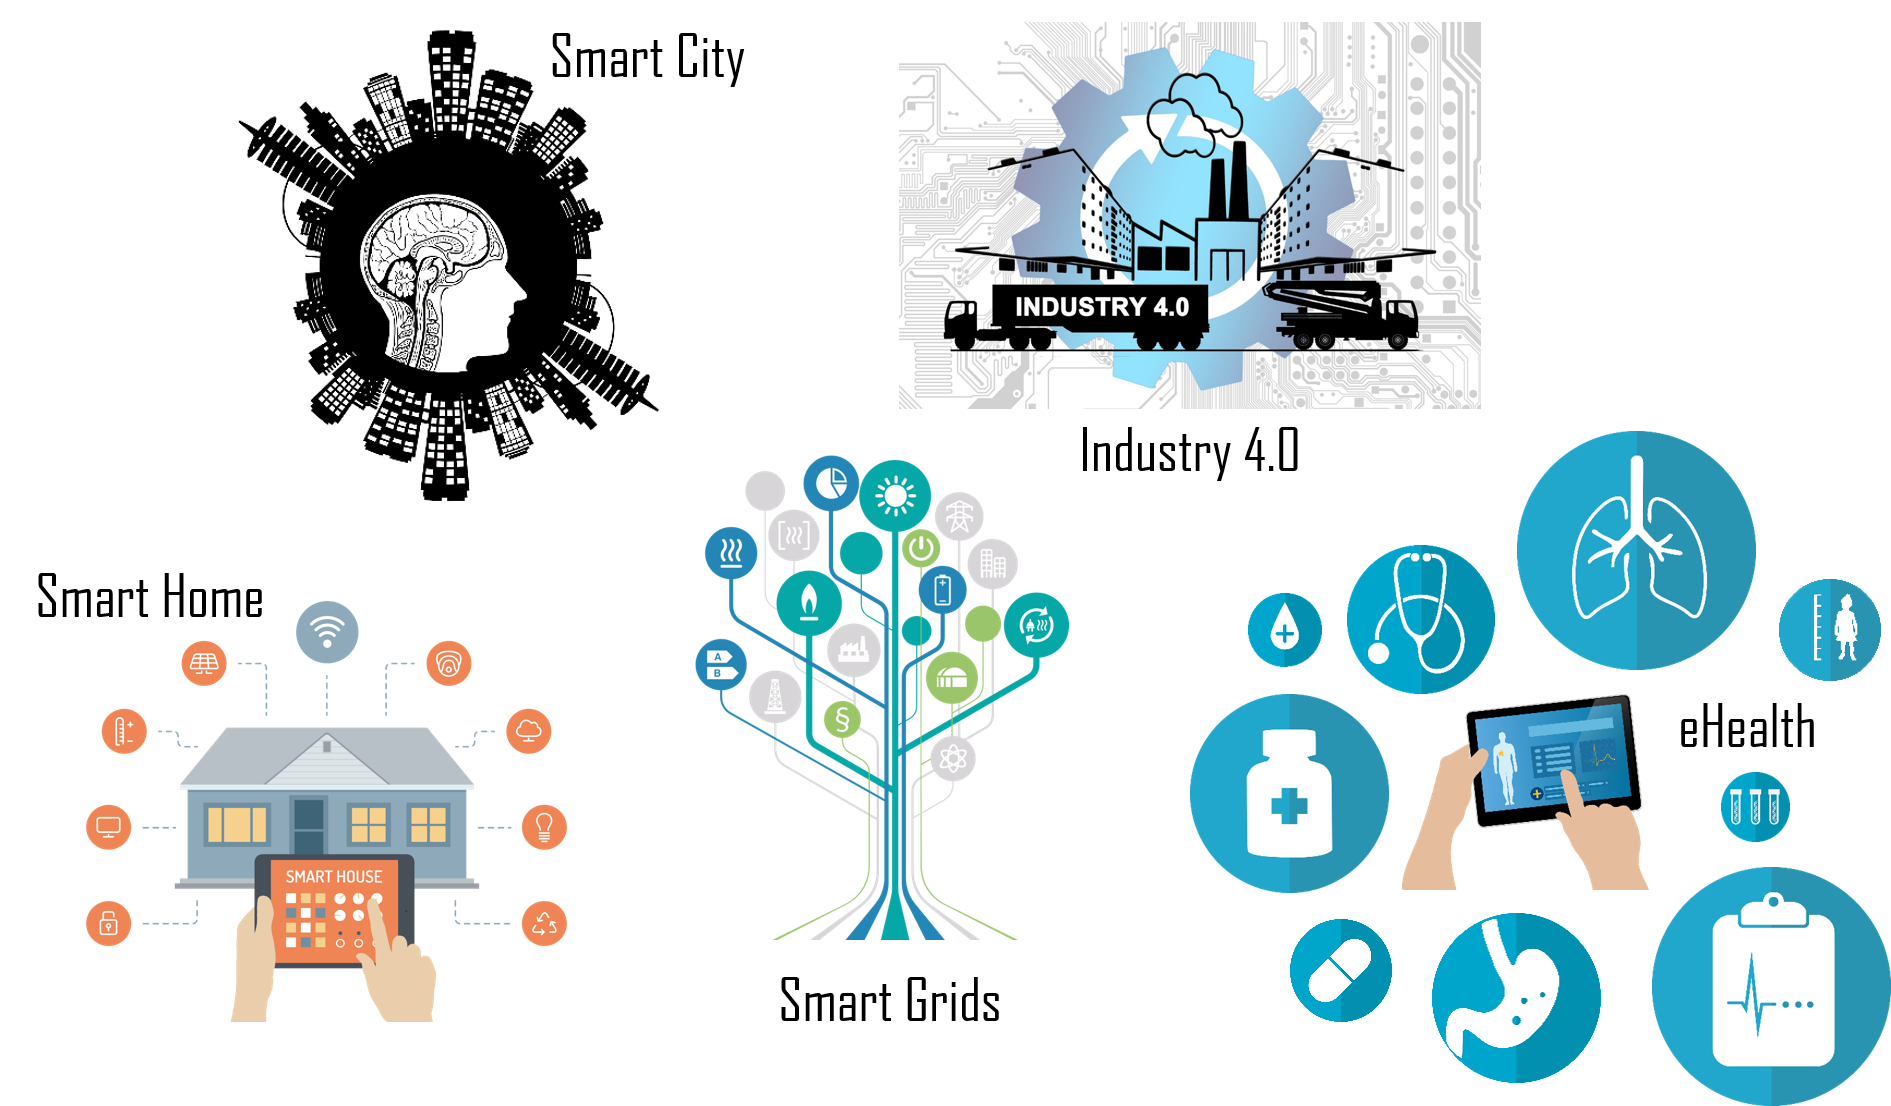
\includegraphics[scale=0.36]{Figures/IoT.png}
    \end{center}
\end{frame}

% % * * * * * * NEW FRAME * * * * * * %
% \begin{frame}{The Internet of Things}
    
% \end{frame}

% * * * * * * NEW FRAME * * * * * * %
\begin{frame}{IoT challenges}
    \begin{center}
        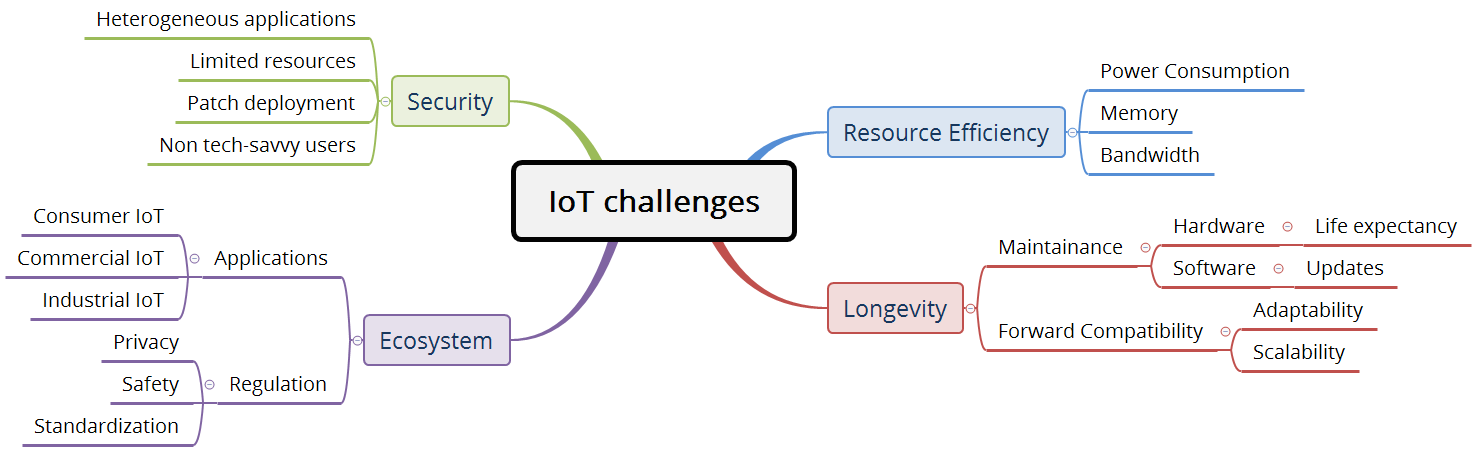
\includegraphics[scale=0.38]{Figures/IoT_challenges.png}
    \end{center}
\end{frame}

\subsection[IoT Security]{The security of the Internet of Things}

% * * * * * * NEW FRAME * * * * * * %
\begin{frame}{Example 1: Animas OneTouch Ping insulin pumps}
    \begin{center}
        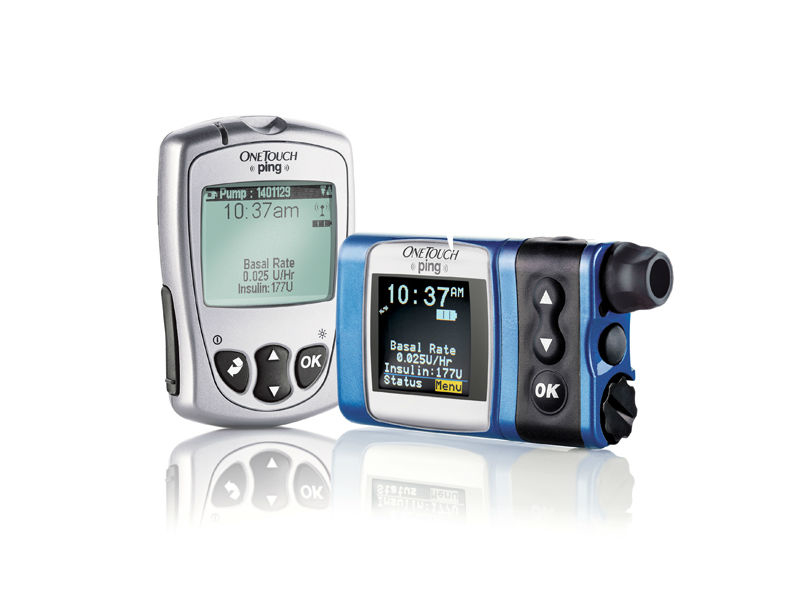
\includegraphics[scale=0.2, trim={0 3cm 0 3cm}, clip]{Figures/insuline_pump.jpg}
    \end{center}
    \vspace{-5mm}
    
    Vulnerabilities:
    \begin{itemize}
        \item Communication in clear
        \item Weak pairing with remote
        \item No replay protection
    \end{itemize}
    
    Attack range:
    \begin{itemize}
        \item 10 m in normal conditions
        \item up to two km with radio equipment
    \end{itemize}
    
    \medskip
    \tiny{Sources: Disclosed by Rapid7 in Oct 2016 \url{blog.rapid7.com/2016/10/04/r7-2016-07-multiple-vulnerabilities-in-animas-onetouch-ping-insulin-pump/}}
\end{frame}

% * * * * * * NEW FRAME * * * * * * %
\begin{frame}{Example 2: 2014 Jeep Cherokee~\cite{miller2015remote}}
    \begin{center}
        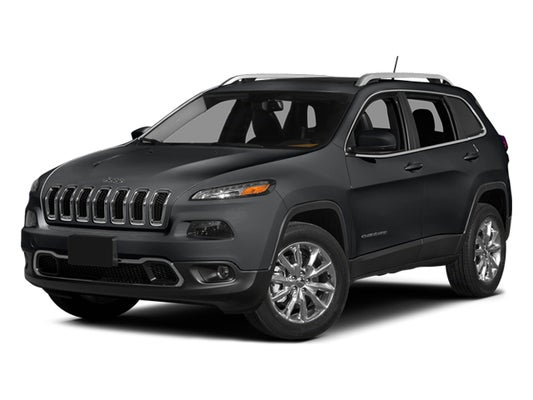
\includegraphics[scale=0.2]{Figures/jeep_cherokee.jpg}
    \end{center}
    \vspace{-5mm}
    
    Effects:
    \begin{itemize}
        \item Switch radio stations and control the volume
        \item Control steering wheel (when the car is slow enough)
        \item Disable brakes (when the car is slow enough)
        \item ...
    \end{itemize}
    
    Attack range:
    \begin{itemize}
        \item from anywhere (over the Internet)
    \end{itemize}
    
    \medskip
    \tiny{Sources: Wired article  \url{https://www.wired.com/2015/07/hackers-remotely-kill-jeep-highway/}}
\end{frame}

% * * * * * * NEW FRAME * * * * * * %
\begin{frame}{Example 3: Mirai Botnet~\cite{antonakakis2017understanding}}

    \begin{center}
        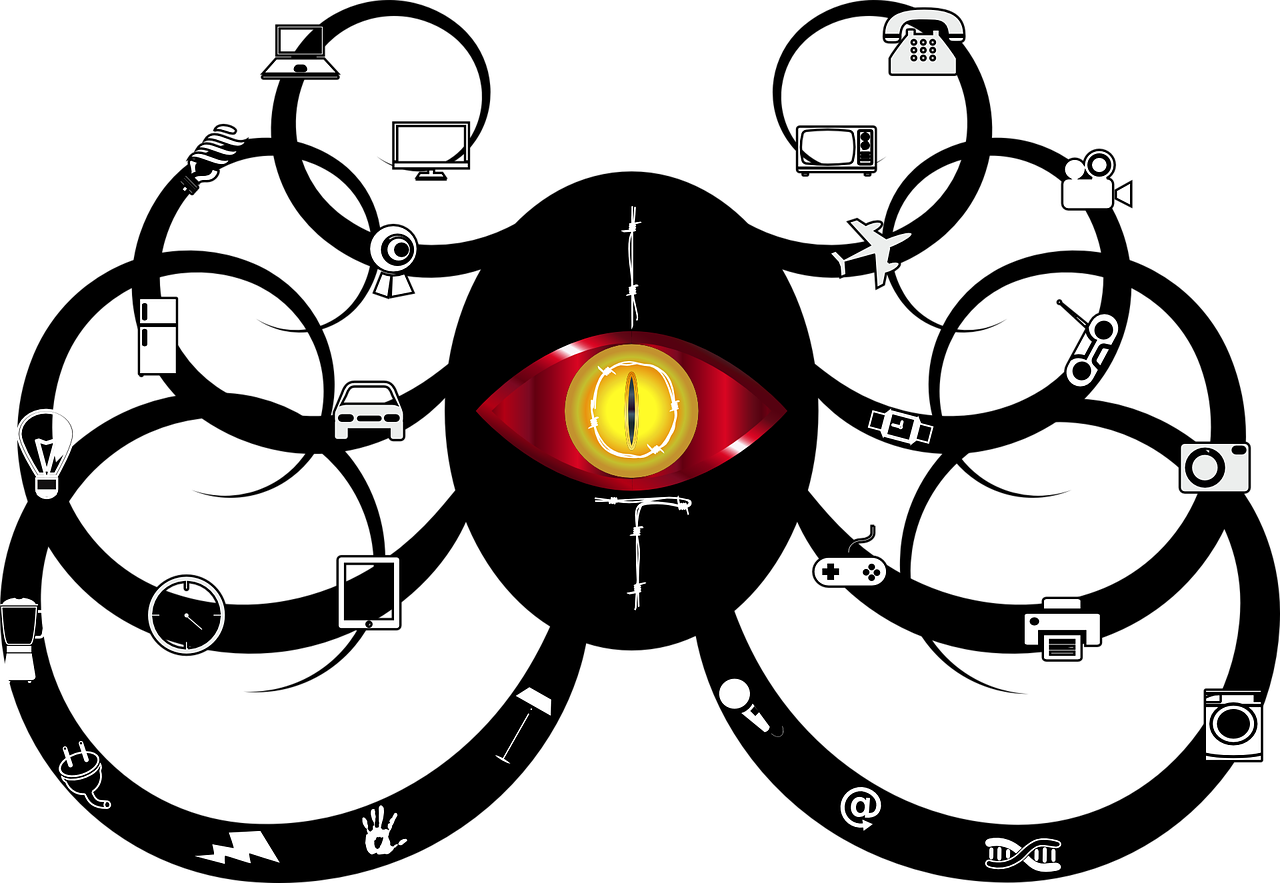
\includegraphics[scale=0.1]{Figures/Miurai_octopus.png}
    \end{center}
    
    Propagation (peaked at 600k hosts):
    \begin{itemize}
        \item Compromised devices scan the network
        \item Devices try login/password from a pre-defined list
        \item Dedicated entity logs in and infects devices
    \end{itemize}
    
    \bigskip
    Targets of Denial of Service attacks:
    \vspace{-3mm}
    \begin{multicols}{2}
        \begin{itemize}
            \item Krebs on security
            \item Dyn
            \item Russian cooking blog
            \item Minecraft servers
        \end{itemize}        
    \end{multicols}
    
\end{frame}

% * * * * * * NEW FRAME * * * * * * %
\begin{frame}{Take away}
    \begin{itemize}
        \item[$\rightarrow$] Many IoT devices are vulnerable because
        \begin{itemize}
            \item Vendors provide optional or inefficient security features
            \item Users fail to configure them
            \item Users fail to update them
        \end{itemize}
        \item[$\rightarrow$] Attacks vary in 
        \begin{itemize}
            \item range
            \item severity
        \end{itemize}
        \item[$\rightarrow$] Attackers can
        \begin{itemize}
            \item compromise people's privacy
            \item affect people's safety
            \item interfere with business activity 
        \end{itemize}
    \end{itemize}
    
    \begin{center}
        \emph{IoT security concerns everyone}
    \end{center}
\end{frame}